\title{ESMValTool-tutorial}
\date{\today}

\documentclass[12pt]{article}
\usepackage{graphicx}
\usepackage[square,comma,numbers,sort&compress]{natbib}
\usepackage[pdfauthor={Martin.Evaldsson@smhi.se},
            pdftitle={ESMValTool Tutorial},
            pdfkeywords={EMBRACE, work package 4},
            pdfsubject={EMBRACE WP 4 visualisation tool}]{hyperref}
\usepackage[hyphenbreaks]{breakurl}
\usepackage[all]{hypcap}
\usepackage{url}
\usepackage{varioref}
\usepackage{multirow}
\usepackage{rotating}
\usepackage{fancyvrb}
\usepackage{color}
\usepackage{amsmath}
\usepackage{appendix}
\usepackage{titlesec}

\definecolor{dark-red}{rgb}{0.4,0.15,0.15}
\definecolor{dark-blue}{rgb}{0.15,0.15,0.4}
\definecolor{medium-blue}{rgb}{0,0,0.5}
\hypersetup{
        colorlinks, linkcolor={dark-red},
        citecolor={dark-blue}, urlcolor={medium-blue}
}

\newenvironment{myverb}{\footnotesize\begin{Verbatim}[frame=single, fontsize=\footnotesize]}{\end{Verbatim}}
%% Define a new 'leo' style for the package that will use a smaller font.
\makeatletter
\def\url@leostyle{%
  \@ifundefined{selectfont}{\def\UrlFont{\sf}}{\def\UrlFont{\small\ttfamily}}}
\makeatother
%% Now actually use the newly defined style.
\urlstyle{leo}

\newcommand{\docref}[1]{`\emph{#1}'}
\newcommand{\xmltag}[1]{\texttt{$<$#1$>$}}

\setcounter{secnumdepth}{5}

\begin{document}
\maketitle

%%%%%%%%%%%%%%%%%%%%%%%%%%%%%%%%%%%
% 
% INTRODUCTION
% 
%%%%%%%%%%%%%%%%%%%%%%%%%%%%%%%%%%%
\phantomsection
\section{Introduction}\label{section:introduction}
The ESMValtool is a software package used to compare and visualize
climate data sets. The tool reads climate data from CMIP5 compliant
netCDF files and generates output in postscript, pdf, png or netCDF.
This document is a revised version of the ESMValTool tutorial given at
the EMBRACE General Assembly in Exeter, June 2013. 

For an overview of the tool, see the slides from the presentation
given at the GA\cite{esmvaltool-presentation} or the
\docref{doc/overview.pdf} document. The tool is directly built upon
the Chemistry-Climate-eValuation Tool\cite{CCMVal-main:2012} (CCMVal
Tool) and the CCMVal reference can provide some background for the
tool.

\paragraph*{Outline:}
The remainder of this document is organized as follows:
section~\ref{section:prerequisites} lists the ESMValTool tutorial
prerequisites, section~\ref{section:overall_structure} gives an
overview of the files and folders of the ESMValTool,
section~\ref{section:running_esmvaltool} details how to run the tool,
section~\ref{section:mydiag} goes through the simplified MyDiag
example, Appendix~\ref{subsection:editable-files} lists the
configuration files and scripts that are edited by the user in the
tutorial `\emph{Try out}'-blocks.

% ############ END OF INTRODUCTION #################


%%%%%%%%%%%%%%%%%%%%%%%%%%%%%%%%%%%
% 
% ESMVAL PREREQUISITES
% 
%%%%%%%%%%%%%%%%%%%%%%%%%%%%%%%%%%%
\phantomsection
\section{ESMVal prerequisites}\label{section:prerequisites}
The ESMValTool requirements are, 
\begin{itemize}
\item{\textcolor{red}{compulsory:}} Python 2.x installation (versions
3.x will not work)

\item{\textcolor{red}{compulsory:}} NCAR Command Language
(NCL)\cite{ncar-ncl-homepage} version 6.1 or higher. Google ``install
ncl'' to find the NCAR page describing how to download and install NCL
locally

\item{\textcolor{red}{compulsory:}} CMIP5-style\cite{pcmdi-cmip5}
netCDF data sets available on the file system. In practice,
``CMIP5-style'' means that some core netCDF attributes are required to
comply with the CF-metadata conventions\cite{pcmdi-cf-conventions}
and, to work work out of the box, the netCDF input file names should
follow the CMIP5-naming convention\cite{DRS-document:2010}. Note that
the tool can be configured to accept non-CMIP5 filenames and to
rewrite non-CF compliant input files on the fly, this is described in
the \docref{doc/reference.pdf}-file. The
\docref{tutorial.tar.gz}\cite{tutorial-tarball} contains a minimal set
of netCDF sufficient for running the examples mentioned in this
document. 

Alternatively, for the better part of the exercises in this document
it is enough to download the following two files from ESGF\cite{esgf}

\begin{Verbatim}[frame=single, fontsize=\footnotesize]
ta_Amon_MPI-ESM-LR_historical_r1i1p1_199001-199912.nc
ta_Amon_MPI-ESM-LR_historical_r1i1p1_200001-200512.nc
\end{Verbatim}

\item{\textcolor{green}{optional:}} The R scripting
language\cite{R-language-ref:2013} version 2.14 or later (older
version may work). R is not needed for the exercises described in this
document, only if the R-based plot scripts are to be used. These plot
scripts does in turn use the following R-packages, 
\begin{itemize}
\item ncdf4
\item fields
\item maps
\item MASS
\item chron
\end{itemize}

\end{itemize}

% ############ ESMVAL TUTORIAL PREREQUISITES #################


%%%%%%%%%%%%%%%%%%%%%%%%%%%%%%%%%%%
% 
% ESMVALTOOL FOLDER STRUCTURE
% 
%%%%%%%%%%%%%%%%%%%%%%%%%%%%%%%%%%%
\phantomsection
\section{ESMValTool folder structure}\label{section:overall_structure}
In a fresh check out from the trunk\cite{ESMValTool_repo} the
following are the most important folders to be aware of,
\begin{Verbatim}[frame=single, fontsize=\footnotesize]
ESMValTool - Earth System Model Validation Tool

For further help, check the doc/-folder for pdfs
and references therein

Important files and folders:
----------------------------

main.py              - Main script

doc/overview.pdf     - Start here if you're new to ESMValTool
doc/*                - Additional documentation for the tool

interface_scripts/   - General Python/NCL routines providing
                       core functionality to the tool
r_code/              - Additional R routines

nml/                 - Implemented namelists for the tool
nml/cfg_*/*          - Diagnostic configuration files

diag_scripts/        - Implemented diagnostics

variable_defs/       - Declaration of all variables and definition 
                       of compound variables

reformat_scripts/    - NCL scripts for reformatting input data files

interface_data/      - Folder for temporary files used to pass in-
                       formation from main.py to the diagnostic
                       scripts
\end{Verbatim}
In addition to the above folders, the
\docref{tutorial.tar.gz}-tarball\cite{tutorial-tarball} includes a
\texttt{Data/}-folder with the CMIP5 data set used to run the example in
this document.

\begin{Verbatim}[frame=single, fontsize=\footnotesize]
ta_Amon_MPI-ESM-LR_historical_r1i1p1_199001-199912.nc
ta_Amon_MPI-ESM-LR_historical_r1i1p1_200001-200512.nc
\end{Verbatim}

To set up the tutorial, issue, 
\begin{Verbatim}[frame=single, fontsize=\footnotesize]
$ svn co --username <USERNAME> <TRUNK-URL> <TARGET-FOLDER>
$ cp tutorial.tar.gz <TARGET-FOLDER>
$ cd  <TARGET-FOLDER>
$ tar xf tutorial.tar.gz
\end{Verbatim}
Alternatively, if the \docref{tutorial.tar.gz} isn't available,
downloading the following two files from ESGF\cite{esgf} is sufficient
for most exercises in this document,

\begin{Verbatim}[frame=single, fontsize=\footnotesize]
ta_Amon_MPI-ESM-LR_historical_r1i1p1_199001-199912.nc
ta_Amon_MPI-ESM-LR_historical_r1i1p1_200001-200512.nc
\end{Verbatim}
Place these files in a local \texttt{Data/}-folder.

% ############ END OF OVERVIEW #################


%%%%%%%%%%%%%%%%%%%%%%%%%%%%%%%%%%%
% 
% ESMVALTOOL LAUNCH COMMAND
% 
%%%%%%%%%%%%%%%%%%%%%%%%%%%%%%%%%%%
\phantomsection
\section{Running the ESMValTool}\label{section:running_esmvaltool}
To run a session of ESMVal, issue 
\begin{Verbatim}[frame=single, fontsize=\footnotesize]
$ ./main.py nml/namelist.xml
\end{Verbatim}
where \texttt{namelist.xml} is any of the namelists in the
\texttt{nml/}-folder. The Python main script will read the namelist
configuration file, e.g., \texttt{nml/namelist.xml}, which contains
sections for \textbf{(a)} global settings, \textbf{(b)} the models
that should be included in this session, \textbf{(c)} a section
listing the diagnostics to plot. These concepts are further explained
in in the following sections.

% ############ END OF LAUNCH COMMAND #################


%%%%%%%%%%%%%%%%%%%%%%%%%%%%%%%%%%%
% 
% MYDIAG EXAMPLE
% 
%%%%%%%%%%%%%%%%%%%%%%%%%%%%%%%%%%%
\phantomsection
\section{The MyDiag template}\label{section:mydiag}
For the purpose of the ESMValTool tutorial a stripped-down and
simplified set of namelist/diagnostics have been prepared. These files
have been designed to let the user play around with the basic features
of the tool without requiring too much knowledge in neither Python,
NCL or the tool design. To be easily recognizable the configuration
files in the MyDiag template have been consistently named: 
\begin{itemize}
\item nml/namelist\_MyDiag.xml, see section~\ref{subsection:mydiag_namelist}
\item variable\_defs/MyVar.ncl, see section~\ref{subsection:mydiag_vardef}
\item diag\_scripts/MyDiag.ncl, see section~\ref{subsection:mydiag_diagnostic}
\end{itemize}

%
%%%%%%%%%%%%%%
% figure: MyDiag example
%%%%%%%%%%%%%%
%
\begin{figure}[!ht]
\begin{center}
\includegraphics[width=0.6\textwidth, angle=90]{figures/MyDiag_MyVar.eps}
\caption{The MyDiag example run ``out-of-the-box''}\label{figure:mydiag_myvar}
\end{center}
\end{figure}
%%%%%%%%%%%%%%
% End of figure
%%%%%%%%%%%%%%

%%%%%%%%%%%%%%%%%%%%%%%%%%%%%%%%%%%
% RUNNING THE MYDIAG EXMAPLE
%%%%%%%%%%%%%%%%%%%%%%%%%%%%%%%%%%%
\phantomsection
\subsection{Running the MyDiag example}\label{subsection:mydiag_testrun}
To run the MyDiag example, make sure the \texttt{Data/}-folder has
been unpacked from the \docref{tutorial.tar.gz}-tarball and is
available in the same folder as the
\texttt{main.py}-script\footnote{Alternatively, use the manual
download approach described at the end of
section~\ref{section:overall_structure}}. Next, issue
\begin{Verbatim}[frame=single, fontsize=\footnotesize]
$ ./main.py nml/namelist_MyDiag.xml
\end{Verbatim}
This will create a new folder specified by the
\texttt{namelist\_MyDiag.xml}\xmltag{plot\_dir}-tag containing a
postscript figure `\texttt{MyDiag\_MyVar.ps}', see
figure~\ref{figure:mydiag_myvar}. The following sections describes the
configuration files/diagnostic scripts that generates this figure. 

%%%%%%%%%%%%%%%%%%%%%%%%%%%%%%%%%%%
% THE MYDIAG NAMELIST
%%%%%%%%%%%%%%%%%%%%%%%%%%%%%%%%%%%
\phantomsection
\subsection{The MyDiag namelist}\label{subsection:mydiag_namelist}
The main configuration file for the ESMValTool is the namelist, the
important sections from the the MyDiag namelist are given below, 
\begin{Verbatim}[frame=single, fontsize=\footnotesize]
<GLOBAL>
    <write_plots type="boolean">           True     </write_plots>
    <write_netcdf type="boolean">          True     </write_netcdf>
    <force_processing type="boolean">     False     </force_processing>
    <wrk_dir type="path">                  work/    </wrk_dir>
    <plot_dir type="path">                plots/    </plot_dir>
    <climo_dir type="path">               climo/    </climo_dir>
    <write_plot_vars type="boolean">       True     </write_plot_vars>
    <max_data_filesize type="integer">      100     </max_data_filesize>
    <max_data_blocksize type="integer">     500     </max_data_blocksize>
    <verbosity  type="integer">               2     </verbosity>
    <exit_on_warning type="boolean">       True     </exit_on_warning>
    <output_file_type>                       ps     </output_file_type>
</GLOBAL>

<MODELS>
    <model>  CMIP5  MPI-ESM-LR   Amon   historical  r1i1p1
                                           1999 2004   Data/  </model>
</MODELS>

<DIAGNOSTICS>
    <diag>
        <description> Textual description of diag </description>
        <variable_def_dir>   ./variable_defs/   </variable_def_dir>
        <variable>             MyVar            </variable>
        <field_type>           T3M              </field_type>

        <diag_script_cfg_dir>./nml/cfg_MyDiag/  </diag_script_cfg_dir>
        <diag_script cfg="cfg_MyDiag.ncl"> 
                                   MyDiag.ncl       </diag_script>
    </diag>
</DIAGNOSTICS>
\end{Verbatim}
The three main sections (tags) listed above are,

\begin{itemize}
\item{\texttt{<GLOBAL>}:} global settings such as \texttt{<plot\_dir>}
- the path to the output figures and \texttt{<output\_file\_type>} - 
the format of the output figures

\item{\texttt{<MODELS>}:} defines which (gridded) data sets should be
used for the diagnostics. In the MyDiag example there is just a single
model defined. The first entry of the \texttt{<model>}-tag,
`\texttt{CMIP5}', indicates that the data set file names should adhere
to the CMIP5 filename syntax\cite{pcmdi-cmip5}. The final
\texttt{<model>}-tag entry defines the full path to the folder with
the input files and the second to the seventh entries are used to
match which files to include.

\item{\texttt{<DIAGNOSTICS>}:} lists which diagnostics, delimited by
the \xmltag{diag}-tags, that should be produced for data sets selected
in the \texttt{<MODELS>}-tag. In this case there is a single
diagnostic defined by the diagnostic script `\texttt{MyDiag.ncl}'
\end{itemize}

\textbf{Try out:} Update some of the global settings, for example
setting the `\texttt{output\_file\_type}' to \texttt{png}, and rerun
the namelist. 

\textbf{Try out:} If you've downloaded additional air temperature
(\texttt{ta}) CMIP5-data sets from ESGF\cite{esgf}, try rerunning
the namelist specifying one of those data set instead of the
MPI-ESM-LR.

%%%%%%%%%%%%%%%%%%%%%%%%%%%%%%%%%%%%%%%%%%
% THE MYDIAG DIAGNOSTIC CONFIGURATION FILE
%%%%%%%%%%%%%%%%%%%%%%%%%%%%%%%%%%%%%%%%%%
\phantomsection
\subsection{The MyDiag diagnostics}\label{subsection:mydiag_diagtag}
The \xmltag{diag}-tags of the \texttt{nml/namelist\_Mydiag.xml}-file
specifies which diagnostic to plot. The \xmltag{diag}-tag given above
is repeated here for convenience,
\begin{Verbatim}[frame=single, fontsize=\footnotesize]
<diag>
    <description> Textual description of diag </description>
    <variable_def_dir>   ./variable_defs/   </variable_def_dir>
    <variable>             MyVar            </variable>
    <field_type>           T3M              </field_type>
    <diag_script_cfg_dir>./nml/cfg_MyDiag/  </diag_script_cfg_dir>

    <diag_script cfg="cfg_MyDiag.ncl"> 
                               MyDiag.ncl       </diag_script>
</diag>
<diag>
\end{Verbatim}

The \texttt{<diag>} tag encloses the following tags,
\begin{itemize}
\item{\xmltag{description}:} a textual summary of the current
\xmltag{diag}-tag

\item{\xmltag{variable\_defs}:} folder where the variable scripts are
located

\item{\xmltag{variable}:} a variable script - the script defines
the variable to plot and if/how it should be transformed prior to
plotting.  See section~\ref{subsection:mydiag_vardef}
for details

\item{\xmltag{field\_type}:} a string describing the required type
of the input field. Here, \texttt{T3M} indicates that the data is a
time series (\texttt{T}), 3-dimensional (\texttt{3}), monthly means
(\texttt{M}).

\item{\xmltag{diag\_script\_cfg\_dir}:} folder where the diagnostic
specific configuration file is located

\item{\xmltag{diag\_script}:} the diagnostic script to execute. The
script should be located in the local \texttt{diag\_scripts/}-folder.
Prior to executing the script the settings in the file defined by the
\texttt{cfg}-attribute is loaded
\end{itemize}

\textbf{Try out:} Try updating the diag\_script configuration file,
`\texttt{cfg\_MyDiag.ncl}' (located in the
\texttt{<diag\_script\_cfg\_dir>}), and rerun the namelist. The comments
in `\texttt{cfg\_MyDiag.ncl}' suggests how to change some values in the
configuration file. Additional options for, e.g. projections, can be
found in the NCL documentation at the NCAR 
homepage\cite{ncar-ncl-homepage}.

%%%%%%%%%%%%%%%%%%%%%%%%%%%%%%%%%%%%%%%%%%
% THE MYDIAG VARIABLE CONFIGURATION FILE
%%%%%%%%%%%%%%%%%%%%%%%%%%%%%%%%%%%%%%%%%%
\phantomsection
\subsection{The MyDiag variables}\label{subsection:mydiag_vardef}
The variable tag in the MyDiag diagnostic configuration file
(section~\ref{subsection:mydiag_diagtag}) is a script that defines the
variable to plot and if/how it should be transformed prior to
plotting. Variable scripts are located in the folder specified by the 
\xmltag{variable\_defs}-tag. In the MyDiag-example the variable is
called `\texttt{MyVar}' and is defined in the script
`\texttt{variable\_defs/MyVar.ncl}':

\begin{Verbatim}[frame=single, fontsize=\footnotesize]
;
;  Requires: ta:*3*
;
variable_info = True
variable_info@derived = True
variable_info@long_name = "air temperature"
variable_info@units = "K"
variable_info@MyDiag_title = "200 hPa"

load "interface_script/add_data_var.ncl"
undef("calculate")
function calculate(index [1] : integer,
                   variable [1] : string,
                   field_number [1] : string)
;;                 return_val [1] : logical
;; Arguments:
;;    index    - index to current infile defined in a
;;               temporary file in the folder 'interface_data'
;;    variable - logical with releveant variable as string attribute
;;    field_number  - string with field number classification
;; Return value:
;;    data_new - logical
local tmp, dum, dimension
begin
    data_new = True
    tmp = read_data(index, "ta", "*3*")
    dimension = 1  ; Level

    ; See ./interface_scripts/extract_data.ncl
    dum = extract_data(index, tmp, dimension, 200., 200.)
    dum@long_name = variable_info@long_name

    ; See ./interface_scripts/add_data_var.ncl
    add_data_var(index, data_new, dum, variable)
    return(data_new)
end
\end{Verbatim}
The important lines from the above script, slightly rearranged, are, 
\begin{enumerate}
\item \texttt{variable\_info = True}\\
The `\texttt{variable\_info}' is a global variable used to control the
logic of the tool

\item \texttt{varable\_info@derived = True}\\
\texttt{derived = True} indicates that the function
\texttt{calculate}, defined in the variable script, should be executed
in order to transform/modify the read netCDF before it is sent to the
diagnostic script

\item \texttt{;  Requires: ta:*3*}\\
This lists the dependencies needed for the
\texttt{calculate}-function. The general syntax is
\footnotesize
\begin{Verbatim}
;  Requires: variable1:field_type1,variable2:field_type2,...
\end{Verbatim}
\normalsize
where  the `\texttt{variable?}' refers to other variables and the
`\texttt{field\_type}' is the field\_type described in
section~\ref{subsection:mydiag_diagtag}. Note that on the
`\texttt{Requires:}'-line the field type allows for wildcards and a
`\texttt{*}' can represent any character. In this particular case
`\texttt{*3*}' could match `\texttt{T3M}', `\texttt{C3M}'
(Climatology), `\texttt{T3D}' (Daily), etc.. If no transfomation is to
be performed the syntax `\texttt{;  Requires:none}' should be used.

\item \texttt{function calculate(index [1] : integer,}\\
The function to transform the requested variable. In the above example
a 2D layer is extracted from a 3D data set.

\item \texttt{tmp = read\_data(index, "ta", "*3*")}\\
Reads data from the netCDF files matched in the MyDiag namelist,
section~\ref{subsection:mydiag_namelist}. The field to read,
3-dimensional air temperature, is encoded in the
\texttt{read\_data}-arguments

\item \texttt{dum = extract\_data(index, tmp, dimension, 200., 200.)}\\
The variable `\texttt{dimension}' is set to match the levels-dimension
of the 3D-data set at hand. `\texttt{200., 200.}' denotes a range along
this dimension, i.e., this line will extract the 200 hPa level. 
\end{enumerate}
To conclude, the MyDiag variable script reads air temperature from
3-dimensional data sets, extracts the 200hPa level and sends it to the
diagnostic script described in section~\ref{subsection:mydiag_diagnostic}.

\textbf{Try out:} Try extracting the 850 hPa level instead of the
200hPa, note that `\texttt{200}' is hardcoded not only in the
`\texttt{extract\_data}'-call but also in the title definition,
`\texttt{MyDiag\_title}'. Because of intermediated file caching of the
variable script output it is necessary to remove the files in the
directory specified by the namelist tag \xmltag{climo\_dir}.
\begin{Verbatim}[frame=single, fontsize=\footnotesize]
rm -f <CLIMO_DIR>-FOLDER
\end{Verbatim}
before rerunning the the updated variable script. 

\textbf{Try out:} Try plotting a different 3D-variable, e.g.,
\texttt{ua} if these have been downloaded separately from
ESGF\cite{esgf}. Proceed by by updating the `\texttt{ta}' on the
\texttt{Requires:}-line and in the \texttt{read\_data(...)}-call +
removing the intermediate file if present. \textbf{NB:} if explicit
contour lines were activated in the `\emph{Try out}' block in
section~\ref{subsection:mydiag_diagtag} these contour lines will have
to be updated to a valid \texttt{ua}-range or inactivated.

\textbf{Try out:} Try using a different variable script, e.g.,
`\texttt{variable\_defs/pr.ncl}' instead of the default
`\texttt{variable\_defs/MyVar.ncl}'. This requires updates to the
\texttt{<variable>} and \texttt{<field\_type>}-tag in the MyDiag
diagnostics (section~\ref{subsection:mydiag_diagtag}). Because of the
way the \texttt{MyDiag}-script is implemented it is also necessary
explictly add the following \texttt{variable\_info}-attributes, 
\begin{Verbatim}[frame=single, fontsize=\footnotesize]
var_att_info@MyDiag_title = "title"
var_att_info@long_name = "long_name"
var_att_info@units = "units"
\end{Verbatim}
to the `\texttt{variable\_defs/pr.ncl}' file\footnote{`\texttt{pr}'-data sets
needs to be downloaded separately from ESGF\cite{esgf}} \textbf{NB:} if
explicit contour lines were activated in the `\emph{Try out}' block in
section~\ref{subsection:mydiag_diagtag} these contour lines will have to be
updated to a valid precip range or inactivated.

\textbf{Try out:} Try using the
`\texttt{variable\_defs/pr\_mmday.ncl}'. This requires similar changes
as the ones above.

%%%%%%%%%%%%%%%%%%%%%%%%%%%%%%%%%%%%%%%%%%
% THE MYDIAG DIAGNOSTIC
%%%%%%%%%%%%%%%%%%%%%%%%%%%%%%%%%%%%%%%%%%
\phantomsection
\subsection{The MyDiag diagnostic script}\label{subsection:mydiag_diagnostic}
The \texttt{<diag\_script>} tag in the MyDiag diagnostic configuration
file (section~\ref{subsection:mydiag_diagtag}) specifies which script
that should be used. The script should be located in the local
\texttt{diag\_scripts/}-folder. Prior to executing the diagnostic
script the selected data sets are sent through, and possibly modified
by, the variable script (section~\ref{subsection:mydiag_vardef}).
Settings for the \xmltag{diag\_script} can be defined in the
configuration file defined by its \texttt{cfg}-attribute.

The MyDiag diagnostic script takes a single model and creates global
contour plot averaged over the years specified in the namelist
(section~\ref{subsection:mydiag_namelist}). The script is a minimalist
example of a diagnostic script where many feautres usually available in
diagnostic scripts are removed.

\textbf{Try out:} Try adding the add years used for averaging to the
main title of the diagnostic script. The years are accessible in the
diagnostic script from the `\texttt{models}'-variable. Use the below
lines to copy the start/end years to a local variable.
\begin{Verbatim}[frame=single, fontsize=\footnotesize]
    start_date = models@start_year(0)
    end_date = models@end_year(0)
\end{Verbatim}
Concatenate the `\texttt{start\_year}'/`\texttt{end\_year}' strings to the
main title by,
\begin{Verbatim}[frame=single, fontsize=\footnotesize]
    res@tiMainString      = MyParam + " (" \
                                    + start_year + "-" \
                                    + end_year   + ")"
\end{Verbatim}
Backslash (`\texttt{\textbackslash}') indicates a continuation line.

\textbf{Try out:} Try adding a loop over models so that multiple
models can be defined in the namelist
(section~\ref{subsection:mydiag_namelist}) and plotted into separate
figures. What is needed to do is
\begin{itemize}
\item{\textbf{(1)}} add models to the namelist, \texttt{namelist\_MyDiag.xml}
\item{\textbf{(2)}} update the \texttt{plot\_script/MyDiag.ncl}-script along
the lines,
\begin{Verbatim}[frame=single, fontsize=\footnotesize]
    do imod = 0, dimsizes(models@name) - 1   ; The loop
        ...
        ;; Model aware output figure name
        outfile = plot_dir + "/" + diag_script + "/MyDiag_"\
                           + variable + models@name(imod)\
                           + "."      + file_type
        ;; Open output figure file
        wks = gsn_open_wks(file_type, outfile)
        ...
        ;; Plot!
        map = gsn_csm_contour_map(wks, data1, res)
        ...
        ;; Delete variables that may be re-used with new size
        delete(A0)
        delete(data1)
    end do  ; End of loop
\end{Verbatim}
\item{\textbf{(3)}} download additional data sets from the ESGF data
nodes\cite{esgf} to get a range of models to loop over.
\end{itemize}

Examples of similar loops can be found in the existing diagnostic
scripts in the diag\_scripts/-folder. \textbf{NB-1:} NCL cannot reuse
variables if they are re-assigned with a different size in a later
loop iteration; these variables has to be deleted with
`\texttt{delete(variable)}'. \textbf{NB-2:} To compare the result of
different data sets it is useful to activate the explicit contour
lines mentioned in the `\emph{Try out}'-block in
section~\ref{subsection:mydiag_diagtag}, otherwise each plot will use
different color ranges.

% ############ END OF MYDIAG EXAMPLE #################


\pagebreak
\appendix
\phantomsection
\section{Appendix}
%%%%%%%%%%%%%%%%%%%%%%%%%%%%%%%%%%%
% 
% APPENDIX: USER EDITABLE FILES
% 
%%%%%%%%%%%%%%%%%%%%%%%%%%%%%%%%%%%
\phantomsection
\subsection{User editable files}\label{subsection:editable-files}
Table~\ref{table:editable-files} in this section summarizes the files
edited by the user in the ESMValTool tutorial. 
\begin{table}[!ht]
\begin{center}
\begin{tabular}{|c|c|}
\hline
\multirow{3}{*}{\texttt{nml/namelist\_*.xml}}      & global settings,\\
                                                   & models,\\
                                                   & diagnostics\\
\hline
\multirow{2}{*}{\texttt{variable\_defs/<VAR>.xml}} & variable transformation (if any),\\
                                                   & variable specific settings\\
\hline
\texttt{nml/cfg\_*/*}                               &  diagnostic script settings\\
\hline
\texttt{diag\_scripts/*}                           &  diagnostic script\\
\hline
\end{tabular}
\caption{Reference table for files updated by the user in the
ESMValTool tutorial}\label{table:editable-files}
\end{center}
\end{table}

% ############ END OF EXISTING DIAGNOSTICS #################

\pagebreak


%%%%%%%%%%%%%%%%%%%%%%%%%%%%%%%%%%%
% 
% BIBLIOGRAPHY
% 
%%%%%%%%%%%%%%%%%%%%%%%%%%%%%%%%%%%
\bibliographystyle{plainnat}
\begingroup
\raggedright
\emergencystretch 1.5em
\bibliography{../common}
\endgroup

\end{document}
